\section{ИССЛЕДОВАНИЕ РАБОТЫ РЕВЕРСИВНОГО СЧЕТЧИКА}

В зависимости от состояний входов возможны следующие режимы
работы реверсивного счетчика:

\begin{itemize}
	\item \textbf{Режим счета} реализуется, когда L=1: при подаче счетных
	импульсов на счетный вход СU происходит увеличение двоичного
	выходного кода, при подаче счетных импульсов на счетный вход CD
	
	\begin{itemize}
		\item Уменьшение, информационные входы D0 – D3 могут находиться в
		любом состоянии, что обозначено в таблице символом ×;
	\end{itemize}

		\item \textbf{Режим параллельной} записи обеспечивается,
		когда L=0, при этом кодовые наборы, установленные на
		информационных входах, повторяются на выходах соответствующих
		разрядов, независимо от состояния счетных входов;
	
		\item \textbf{Сброс счетчика} осуществляется подачей высокого уровня
		напряжения на вход R, что приводит к отключению всех других
		входов и запрещению записи. В результате на информационных
		выходах устанавливаются сигналы Qn=0 (n = 0, 1, 2, 3), на выходе
		окончания счета на увеличение — сигнал PU = 1, а сигнал на выходе
		окончания счета на уменьшение PD дублирует состояние счетного
		входа СD. Во всех других режимах R = 0.


\end{itemize}

\begin{figure}[H]
	\centering
	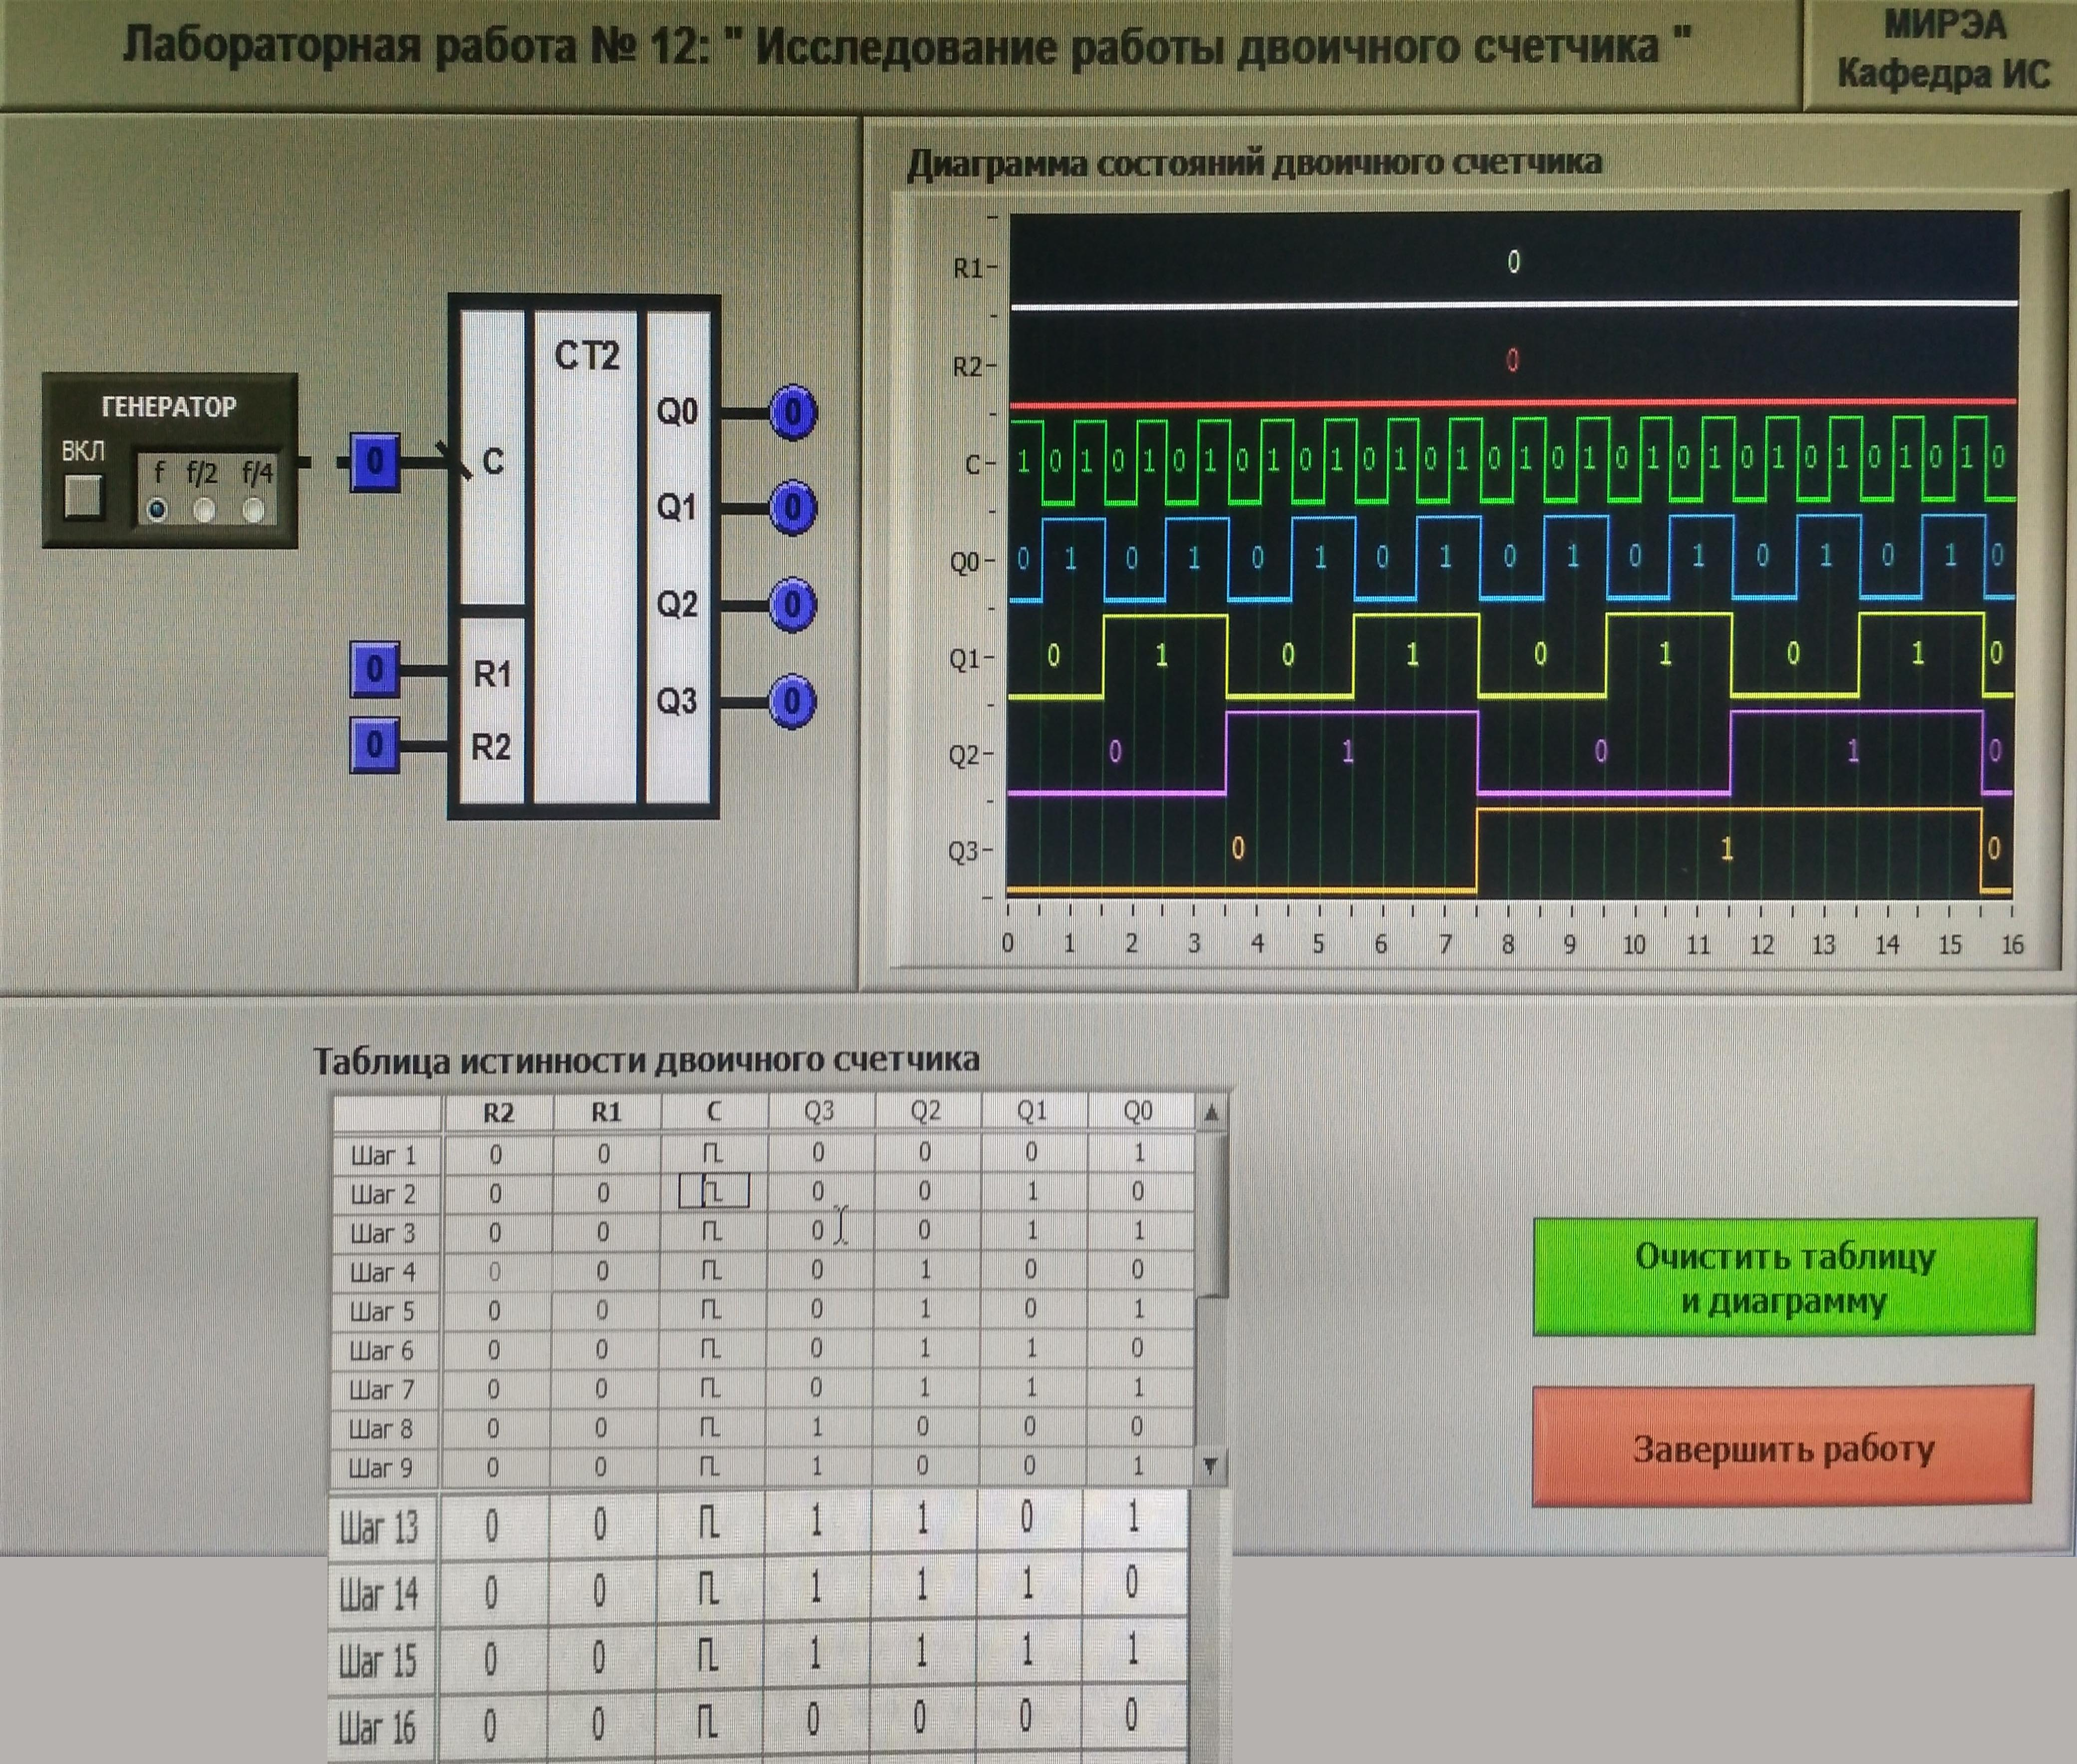
\includegraphics[width=0.95\linewidth]{imgs/14/1.jpg}
	\caption{РЕЖИМ СЧЕТА НА УВЕЛИЧЕНИЕ}
	\label{fig:14_1}
\end{figure}

\begin{figure}[H]
	\centering
	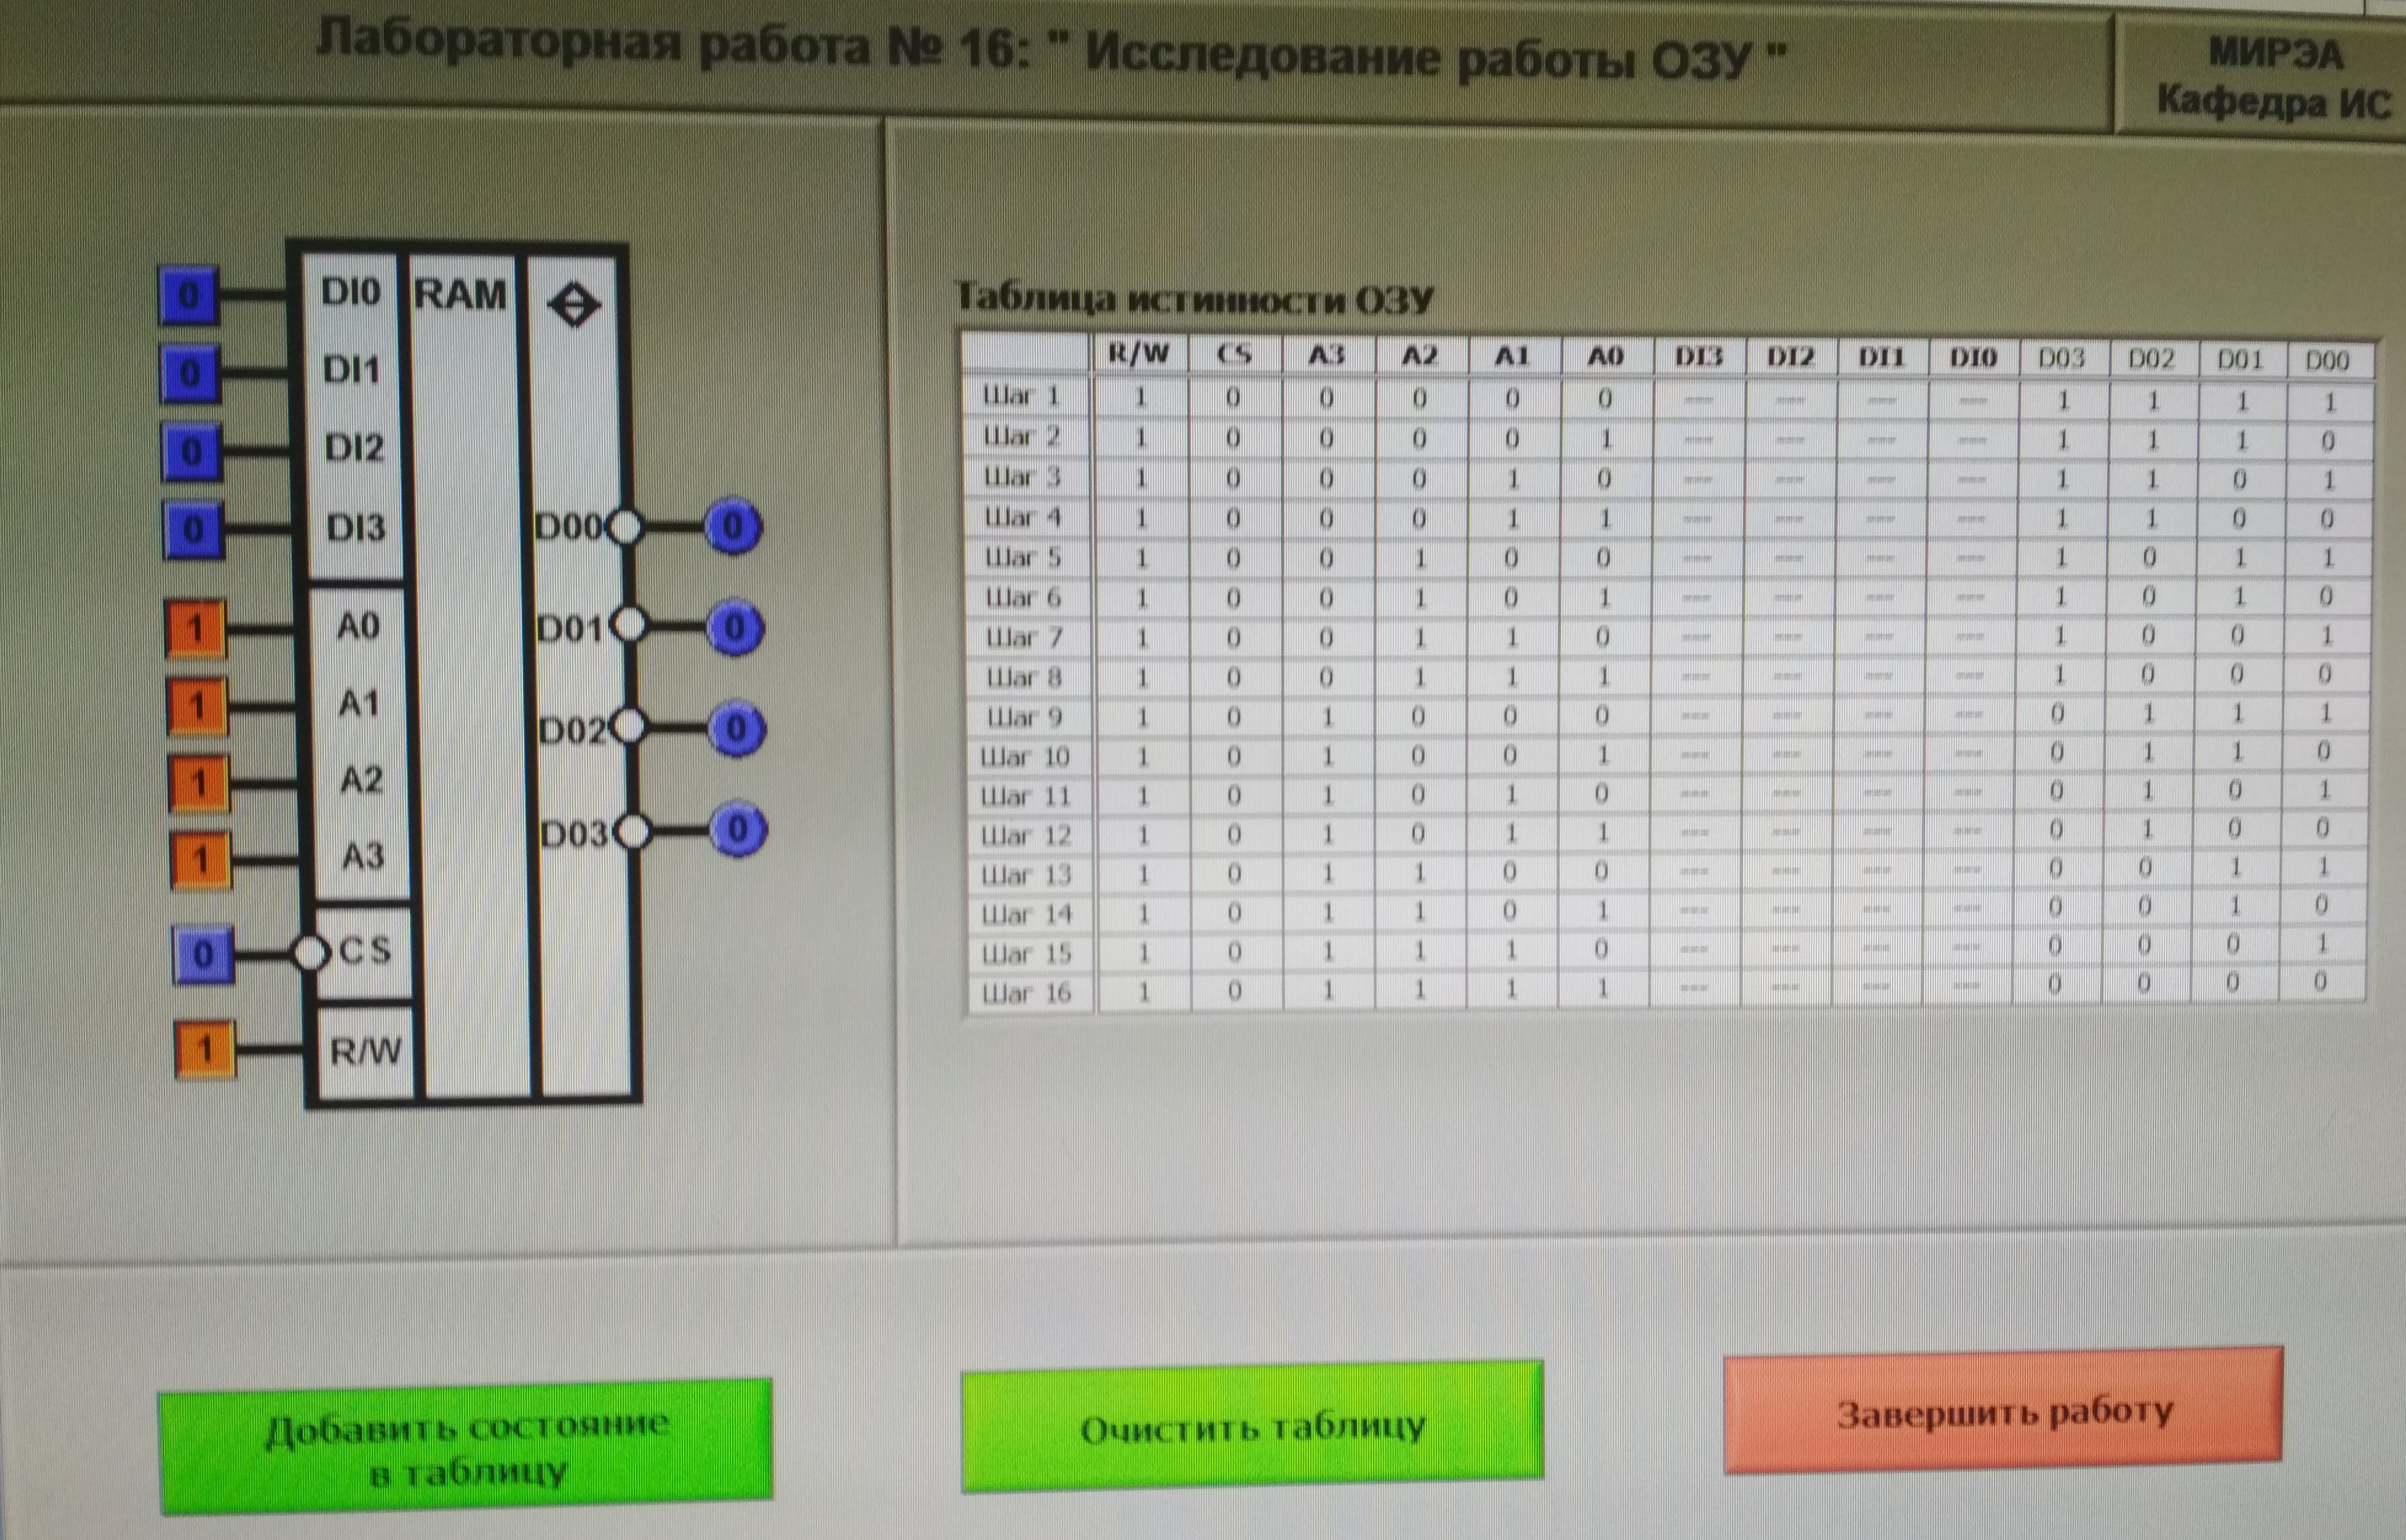
\includegraphics[width=0.95\linewidth]{imgs/14/2.jpg}
	\caption{РЕЖИМ СЧЕТА НА УМЕНЬШЕНИЕ}
	\label{fig:14_2}
\end{figure}

\begin{figure}[H]
	\centering
	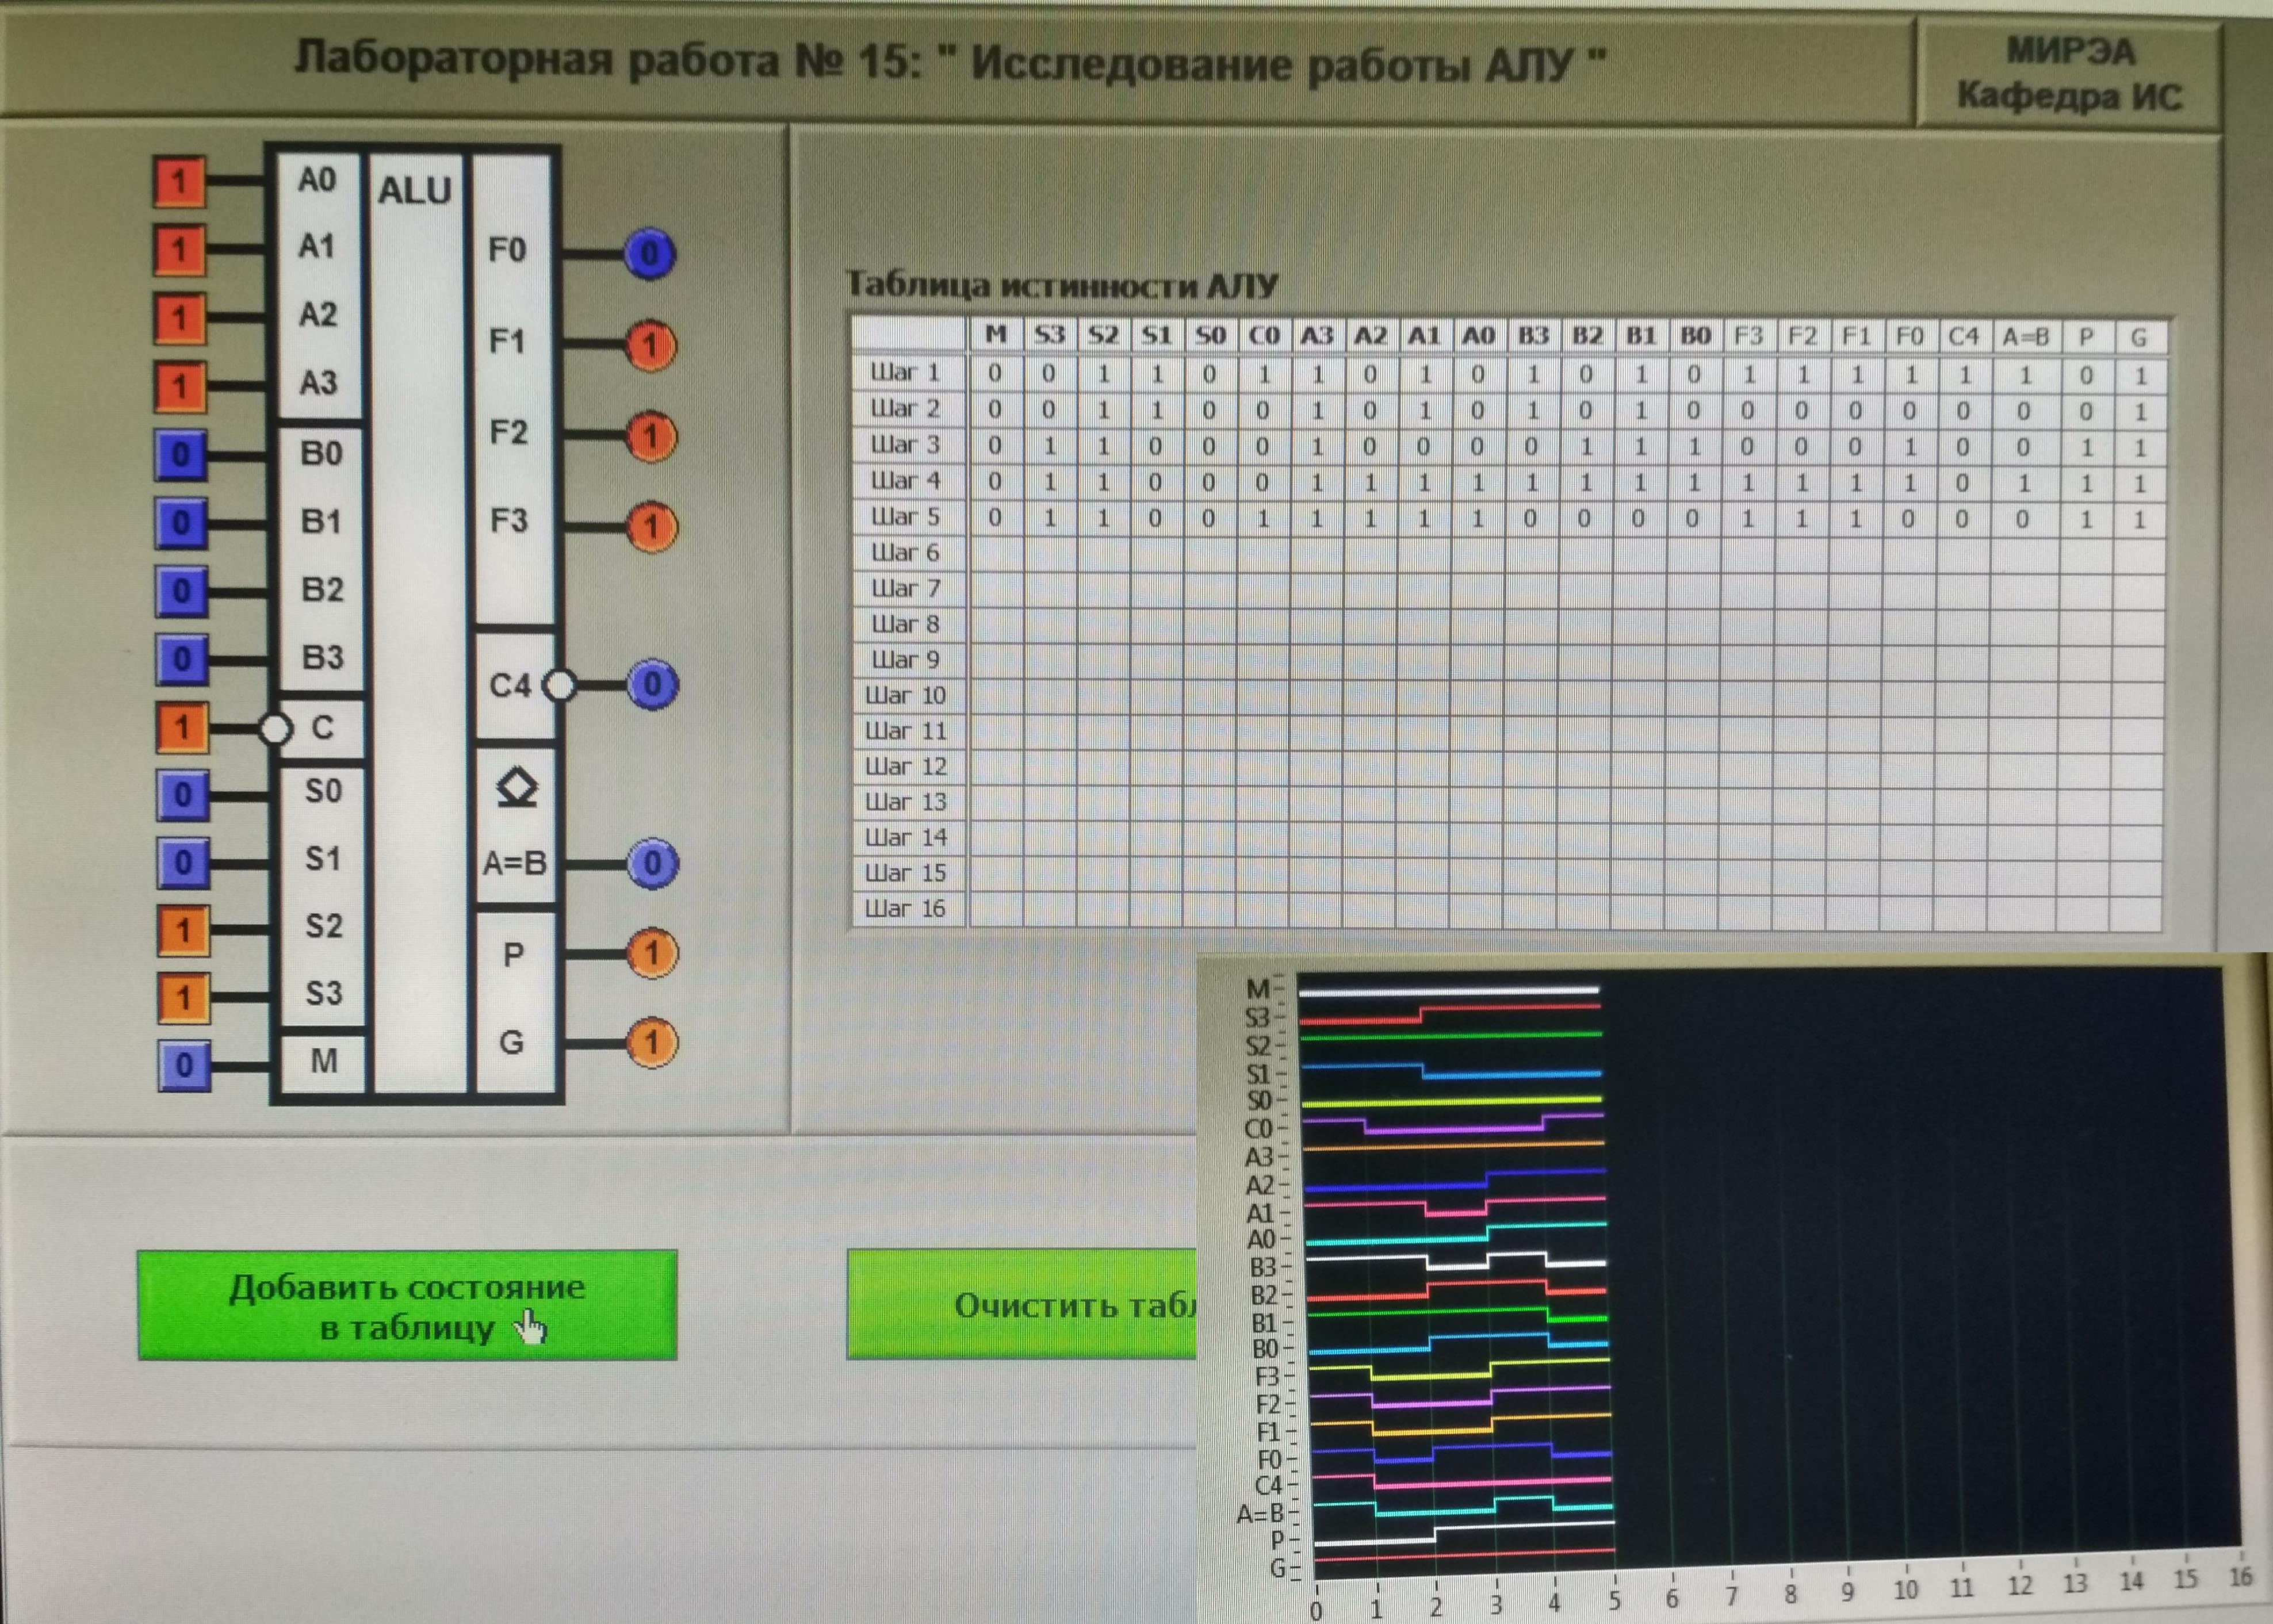
\includegraphics[width=0.95\linewidth]{imgs/14/3.jpg}
	\caption{РЕЖИМ ПАРАЛЛЕЛЬНОЙ ЗАГРУЗКИ}
	\label{fig:14_3}
\end{figure}

\begin{figure}[H]
	\centering
	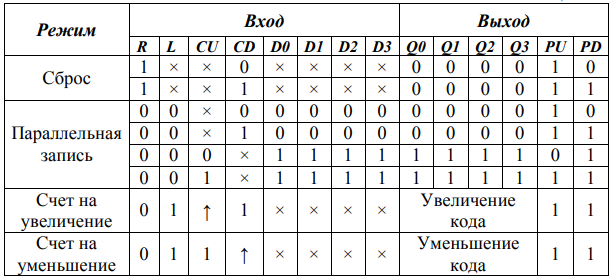
\includegraphics[width=0.85\linewidth]{imgs/14/14_tab}
	\caption{Режим работы сумматора}
	\label{fig:14_tab}
\end{figure}

Элемент SN74LS193 - Low-Voltage BiCMOS Technology

Характеристики:

\begin{figure}[H]
	\centering
	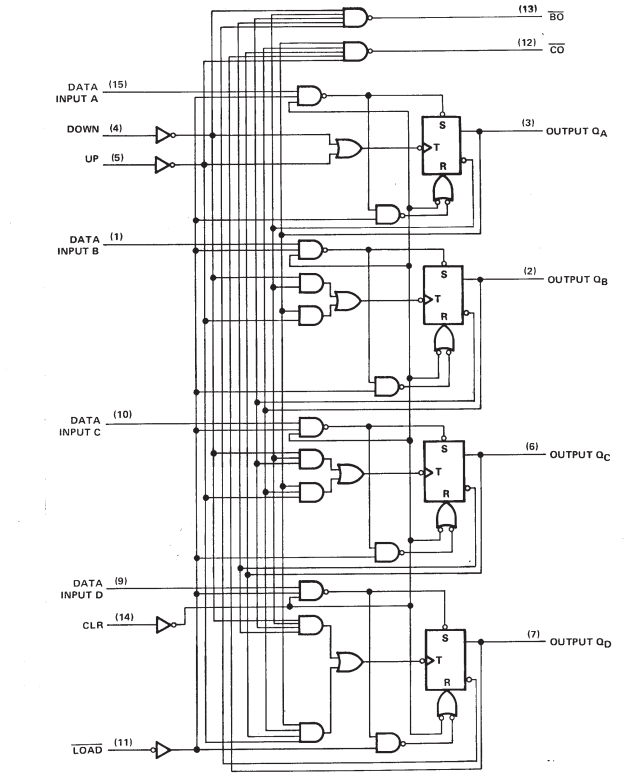
\includegraphics[width=0.95\linewidth]{imgs/14/14_sh}
	\caption{Схема}
	\label{fig:14_sh}
\end{figure}

\begin{figure}[H]
	\centering
	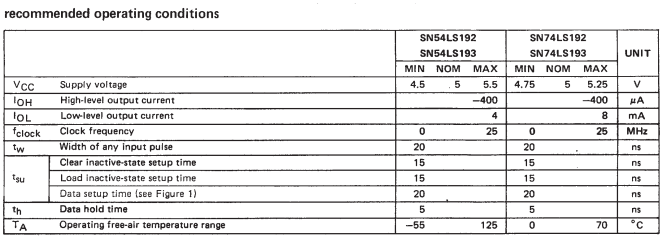
\includegraphics[width=0.95\linewidth]{imgs/14/14_rec}
	\caption{Рекомендуемые параметры}
	\label{fig:14_rec}
\end{figure}

\begin{figure}[H]
	\centering
	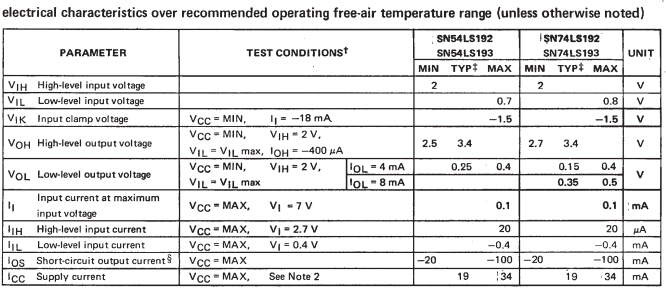
\includegraphics[width=0.95\linewidth]{imgs/14/14_ch}
	\caption{Электрические характеристики}
	\label{fig:14_ch}
\end{figure}

\begin{figure}[H]
	\centering
	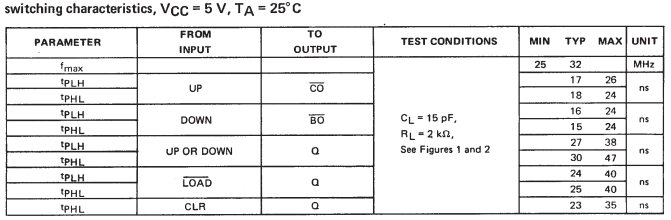
\includegraphics[width=0.95\linewidth]{imgs/14/14_switch}
	\caption{Коммутационные характеристики}
	\label{fig:14_switch}
\end{figure}
